\chapter[Microscope deux photons rotatif]{Microscope à feuille de lumière deux photons rotatif}\label{chapIV}

% OK VolkerComment
% General remark: Everything that I discussed about the fibers in my first version of the manuscript has to be discussed in your thesis. And you have to extend this and go beyond this and not give less details and less citations.

% OK VolkerComment
% You have to extend significantly this introduction and link it to the previous chapters. Your aim was to perform the multisensory virtual reality experiments that you described in in Chapter 1 while recording whole brain activity. Two further developments of Geoffrey's setup where necessary
% 1. You needed a system that allows to stimulate the tilt direction.
% 2. You needed a two-photon system to gain high control over the visual stimulus.
% Start with the description to the tilt setup that you developed with Thomas Panier. You can first present it as a one-photon system, talk about the differences in the optical path, the different motor, your control software, the mechanical stability characterization and finish with recordings in one-photon mode. Use the figures of the schematic of the setup and of the one-photon tilt phase maps from the Brighton poster. Then you talk about the transformation of the system into a two-photon setup and the challenge of fiber coupling the two photon laser ... . Here you have to introduce the demands on the fiber coupling properties necessary to develop successfully a 2PRLS. :
% (i) High power transmission and damage threshold
% (ii) low dispersion
% (iii) polarization maintenance
% (iv) low bending loss
% (v) single mode maintenance during bending
%
% [rephrased]
% postural control in virtual environment -> under microscope
% - tilt direction stimulation
%   - differences in optical path
%   - motor
%   - control software
%   - mechanical stability characterization
%   - one photon recordings
%   - brighton phasemaps
% - two-photon system for visual control
%   - fiber coupling
%   - dynamic effects...
%   

% Pour étudier à la fois le système visuel et le système vestibulaire du poisson zèbre, une possibilité est de combiner les deux innovations précédemment citées en un seul microscope : un microscope à feuille de lumière deux photons rotatif. C'est la voie que j'ai explorée, qui a révélé plusieurs défis techniques. Le premier et de guider le laser deux photons vers le module light-sheet en restant stable lors de la rotation du microscope. Le second est de mitiger l'effet de lentille thermique lié à la propagation d'un faisceau haute puissance dans l'eau. Après avoir exploré en détail ces aspects techniques, je montrerai comment le microscope a permis de réaliser l'acquisition du cerveau de la larve sans environnement visuel parasite.


% OK Volker (à propos de la décroissance de l'intensité dans la direction de propagation)
% Show an image. Is this really an issue. The infrared light interacts less with the tissue compared to the 488nm laser. How do both configurations compare? I do not see uneven fluorescence signal across the fish in two photon recordings.

Pour réaliser l'imagerie du cerveau lors du contrôle postural tel que présenté au chapitre \ref{chapII}, il faut contrôler à la fois l'environnement visuel et l'environnement vestibulaire.
Dans le chapitre \ref{chapIII}, je présente un microscope rotatif capable d'imager le fonctionnement du cerveau lors d'une stimulation vestibulaire réelle, ce qui répond en partie au problème. Dans ce chapitre, je m'intéresse à l'autre partie : comment réaliser l'imagerie tout en contrôlant l'environnement visuel, et cela en même temps qu'une stimulation vestibulaire.

% IGN VolkerComment2
% Change the structure: Talk first about the solution by Vladimirov and then introduce the alternative approach of 2P imaging. In this way you can explain the two photon part step by step from standard 2P scanning microscopy (here you explain the principle) to 2P light-sheet microscopy (here you have to introduce the high laser power required for fast functional 2P light-sheet imaging). Then discuss the challenge of fiber coupling a two photon laser necessary for the development of a rotating 2P microscope (dispersion, non-linear effects at laser powers > 10mW ..., fiber damage). Then write that the field of imaging in freely moving rats with head mounted fiber scopes faces the same challenge. Now introduce fiber light guides in general and then introduce step by the different solutions found in the literature : 1. Precompensation, 2. hollowcore fibers (i. photonic bandgap fibers). Discuss directly in each subsection the applications and the limitations of the solutions (low laser power transmission, single wavelength and not at 930nm ...) . Then finish with a statement that states that broadband fiber coupling with >90% transmission would be desirable. Start a new chapter and present your work with Kagome and NCF fibers. (1) start with the history and the general properties of these fibers. (2) Explain why you selected the fiber that we use now and show the characterization provided by GLO (3) Then continue with you fiber coupling part, (4) introduce the necessity of the NA expander and how you implemented it, (5) discuss your M2 value characterization at the fiber output and the measured beam profile, (6) show that your system can perform high resolution anatomical brain scans in one- and two-photon mode (this figure is currently missing in your manuscript). Now start a new section and discuss the atifact when you rotate the system. Now you describe step by step how you optimized the system to reduce all artifacts (1) bending loss (2) circular polarization (3) average laser power ....

% vladimirov
% 2P imaging
% challenge 2P fiber
% freely moving rats
% fiber light guides
% precompensation / HCF
% NCF 1) history 2) why this one 3) coupling 4) NA exp 5) M² 6) brain scan
% artifacts 1) bending loss 2) circular polar 3) average power


Un microscope à feuille de lumière classique utilise un laser bleu pour stimuler la fluorescence, et cette longueur d'onde réside dans le domaine visible de la larve de poisson zèbre, ce qui peut l'éblouir et perturber son système visuel. Pour cette raison, Ahrens \emph{et al}, pour l'étude de la réponse optomotrice, ont utilisé un microscope à deux photons classique \cite{ahrens_brain-wide_2012}. Cela permet d'illuminer dans l'infrarouge, une longueur d'onde invisible pour le poisson. Cependant ils ne bénéficiaient pas des avantages d'un microscope à feuille de lumière et étaient contraints par le balayage point par point à réaliser l'acquisition du cerveau une région après l'autre afin de reconstruire \emph{a prosteriori} l'image du cerveau entier. À peu près en même temps, Truong \emph{et al} publiaient un microscope à feuille de lumière deux photons permettant d'allier les avantages de la microscopie deux photons et de la microscopie à feuille de lumière \cite{truong_deep_2011}.

% IGN VolkerComment2
% "avantages" -> specify the advantages again here.
% Truong:
% Their main focus was to increase penetration depth in not fully transparent samples as a Drosophila larva in the context of volumetric live imaging during development. Compared to functional whole-brain imaging in zebrafish larvae they do very slow imaging. They demonstrated that two-photon light sheet microscopy is possible. And that the high laser power required does not burn the sample. As a major result they demonstrate that they can penetrate two time more the sample due to less scattering of IR laser, 2P effect reduces fluorescent excitation by scattered light, reduced autofluorescence at IR wavelength. FYI: here also the patent with interesting discussions https://patents.google.com/patent/US8441633B2/en

% IGN VolkerComment2
% Vladimirov
% Show the figure that demonstrates the configuration of the two light-sheets

% IGN VolkerComment5
% Truong et al used the 2P for structural imaging. Wolf observed that you can use it also in the context of functionnal brain imaging with much higher required volumetric recording rates and so higher laser power and that you do not burn the fish

Plus tard, Vladimirov \emph{et al} \cite{vladimirov_light-sheet_2014} ont montré que l'étude de l'OMR était également possible en microscopie à feuille de lumière un photon, à condition de ne pas éclairer directement l'œil du poisson. Ils ont utilisé deux feuilles de lumière, l'une éclairant le cerveau par le côté et l'autre par l'avant, entre les deux yeux. Cependant, l'OMR est un réflexe robuste qui ne recourt pas aux fonctions avancées de la vision, et la perturbation due à l'illumination des autres processus visuels n'est pas contrôlée. C'est pourquoi Wolf \emph{et al} ont appliqué la technique mise au point par Truong à l'étude du système visuel de la larve de poisson zèbre \cite{wolf_whole-brain_2015}. Ils ont construit un microscope à feuille de lumière deux photons et réalisé l'acquisition du cerveau entier lors de stimulations visuelles.

% IGN VolkerComment2
% Discuss the paper: They demonstrated lower visual response threshold in 2P LSM compared to 1P LSM. Show the figure 1b of Wolf et al. Discuss also that one cannot image through the eyes as this will burn the fish.

Pour étudier le cerveau lors du contrôle postural, il est donc nécessaire de réaliser un microscope rotatif deux photons, ce qui soulève plusieurs enjeux techniques. D'une part, pour guider le laser d'excitation vers une plateforme mobile, il faut disposer d'une fibre adaptée (transmission de grandes puissances, faible dispersion, maintien de la polarisation, faibles pertes de courbure), d'autre part il faut minimiser les effets dus à la propagation d'un faisceau intense dans un fluide en mouvement. Ce chapitre débute sur les fibres optiques adaptées à la transmission d'un laser pulsé et leur utilisation en microscopie embarquée, et poursuit sur la construction d'un microscope deux photons rotatif fibré.

% TOOD VolkerComment2
% (grandes puissances)
% You have to introduce and discuss the high laser power requirement for 2P LSM in you intro.


\section{Effet deux photons}

\subsection{Principe}

L'absorption deux photons est un phénomène non linéaire d'absorption simultanée de deux photons par une molécule ou un atome. Cet effet est proportionnel au carré de l'intensité lumineuse incidente et est lié au caractère anharmonique du dipôle oscillant. Pour cette raison, il est négligeable aux petites énergies mais devient important pour une intensité lumineuse élevée. On peut l'observer en concentrant fortement un faisceau puissant. La concentration peut être à la fois spatiale par focalisation et temporelle par impulsion temporelle.

\subsection{Concentration spatiale}
 
Un système optique peut concentrer la lumière localement, ce qui produit un point de plus grande intensité, le point focal. Comme l'effet deux photons est proportionnel au carré de l'intensité, la zone concernée est d'autant plus restreinte. Cette propriété est utilisée en microscopie multiphoton pour produire une illumination ponctuelle qui permet le sectionnement optique dans la direction de propagation. En microscopie à feuille de lumière, au contraire, une illumination linéaire est recherchée. La focalisation est donc bien moindre et l'effet deux photons contribue à affiner la zone d'excitation, la fluorescence n'étant excitée qu'au centre du faisceau (Fig. \ref{FIG2P-intensity-profile}).

% IGN VolkerComment2
% You have to make a figure. Show the Jablonski diagram and e.g. this https://www.researchgate.net/figure/Two-photon-fluorescence-vs-normal-fluorescence-The-blue-scanning-laser-in-the-left_fig11_326583720. Discuss that via the two photon effect you can excite the same fluorophore (GCaMP) with an IR laser of double the wavelength compared to the one photon case. In this configuration you laser is outside the sensitive spectrum of the fish retina.
% Is linear the correct word? An extended focus is needed to create the light-sheet

\begin{figure}[p]
    \centering
    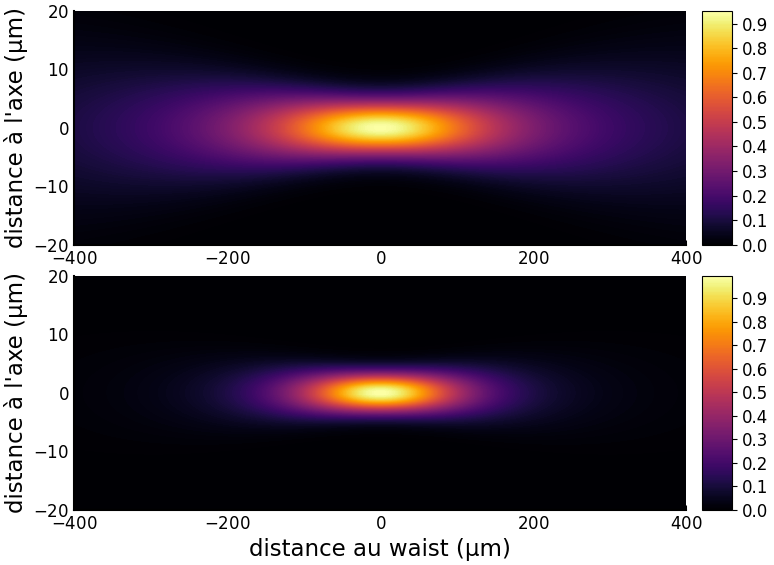
\includegraphics[width=0.8\textwidth]{./files/profile-intensity.png}
    \caption{Effet deux-photons en microscopie à feuille de lumière. Comparaison du profil d'intensité (haut) et de son carré (bas). On voit que la zone concernée par l'effet deux photons est restreinte, ce qui permet d'obtenir un sectionnement vertical comparable à la feuille de lumière 1P malgré une longueur d'onde plus élevée. On voit aussi que l'intensité décroit plus vite dans la direction de propagation, ce qui diminue le signal sur les bords du cerveau. (paramètres : indice optique 1.33, longueur d'onde 915 nm, waist 6.5 µm)}
    \label{FIG2P-intensity-profile}
    \end{figure}

\begin{figure}[p]
    \centering
    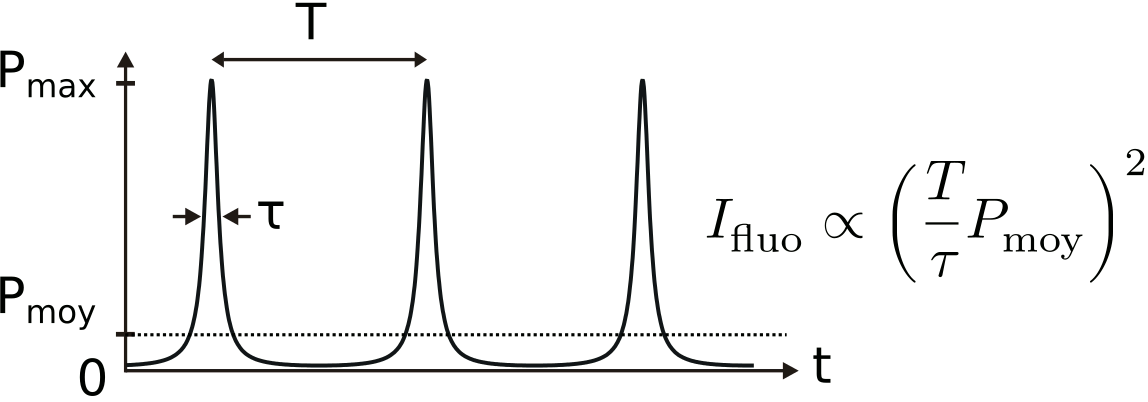
\includegraphics[width=\textwidth]{./files/pulsed_laser.svg.png}
    \caption{Profil temporel de puissance d'un laser pulsé. Chaque impulsion a une durée $\tau$, elles sont espacées d'une durée $T=1/f$, où $f$ est la fréquence de répétition du laser. À puissance moyenne $P_\text{moy}$ constante, plus $\tau$ est petit, et plus $T$ est grand, plus la puissance maximale $P_\text{max}$ est grande. L'intensité de fluorescence en deux photons est proportionnelle au carré de $P_\text{max}$ alors qu'elle est proportionnelle à $P_\text{moy}$ en un photon.
    }
    \label{FIGpulsed-laser}
    \end{figure}

\subsection{Concentration temporelle}\label{SECTIONconcentrationtemporelle}
    
Une autre manière de concentrer la lumière est la concentration temporelle. Dans le cas d'un laser continu, la puissance est répartie sur toute la longueur de propagation du faisceau. En utilisant un laser pulsé, la puissance est concentrée en paquets beaucoup plus courts (Fig. \ref{FIGpulsed-laser}). Par exemple, pour des impulsions de 100 fs, malgré la vitesse élevée de la lumière, la longueur de ces paquets est de 30 µm (100e-15 $\times$ 3e8 = 3e-5). Si de plus le taux de répétition du laser est de 80 MHz, la puissance d'une impulsion est 125 fois plus élevée qu'un laser continu de même puissance moyenne (1/(100 fs $\times$ 80 MHz)). L'effet deux photons étant proportionnel au carré de la puissance instantanée, on a intérêt à choisir les impulsions les plus courtes possibles (petit $\tau$) et le taux de répétition le plus faible possible (grand T) pour un laser de puissance moyenne fixée \cite{maioli_fast_2020}. Cette tendance est limitée par les photoperturbations induites, qui deviennent importantes au-delà d'une centaine de nanojoules par impulsion. Pour Gasparoli \emph{et al}, les conditions optimales en microscopie par fluorescence à nappe laser deux photons sont f = 1 MHz, $\tau$ = 100 fs, P = 100 mW, $\lambda$ = 920 nm \cite{gasparoli_is_2020}. Pour Maioli \emph{et al}, elles sont de f = 10 MHz, $\tau$ = 300 fs, P = 70 mW, $\lambda$ = 1030 nm \cite{maioli_fast_2020}.

% Cependant, ces derniers suggèrent de repousser la longueur d'onde vers les 1100 nm pour réduire l'absorption. (cf partie lentille thermique)

% OK VolkerComment2
% Move this to the discussion. Also from where do you get the numbers? citation is missing. Willy Supatto shows in his 2020 paper that 10MHz is the optimal repetition rate.


\section{Fibre optique, principe et état de l'art}

Pour obtenir un bon signal de fluorescence par excitation à deux photons, il est donc nécessaire de transmettre jusqu'à l'échantillon un faisceau à haute puissance tout en conservant des impulsions courtes. Les fibres classiques comme celle utilisée dans la version un photon du microscope n'ont pas ces propriétés et il faut donc s'intéresser aux mécanismes du guide d'onde pour trouver une solution à ce problème.

\begin{figure}
    \centering
    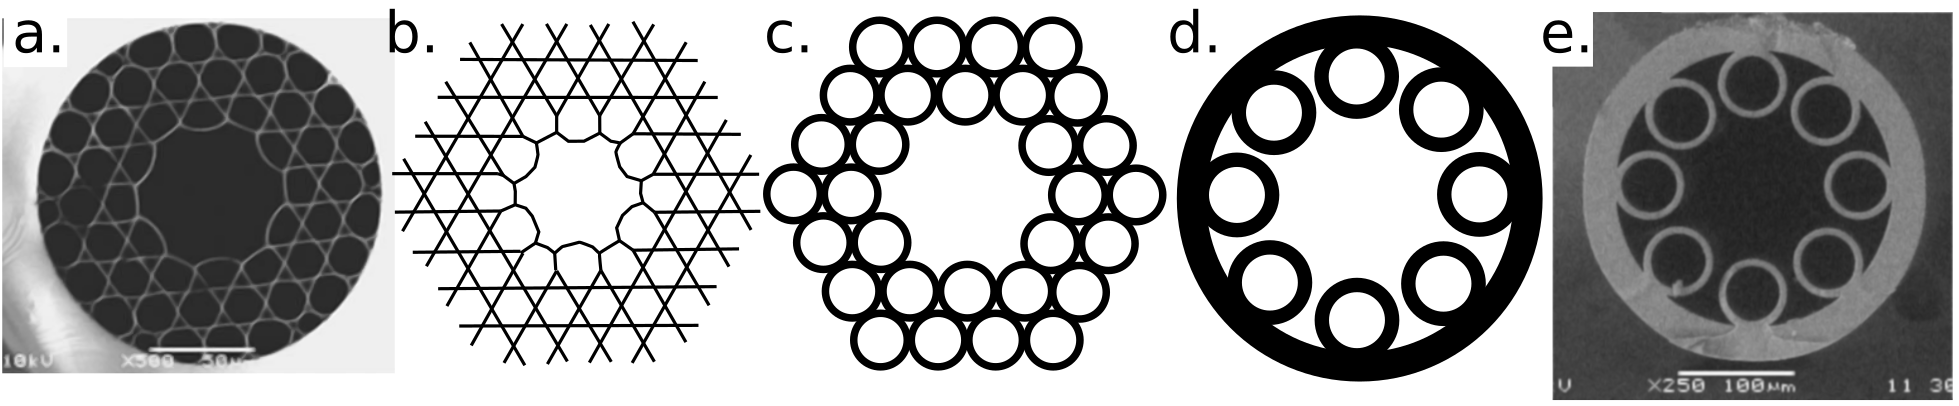
\includegraphics[width=\textwidth]{./files/fibers.svg.png}
    \caption{Aperçu sur les fibres et exemples de fibres à cœur creux évoquées dans le texte.
    \\ a1. Fibre Kagomé (image extraite de Wang 2011 \cite{wang_low_2011}), schéma du motif en a2.
    \\ b1. Fibre à réseaux de tube (image extraite de Cregan 1999 \cite{cregan_single-mode_1999}), schéma du réseau tubulaire comme dans Vincetti 2010 \cite{vincetti_waveguiding_2010} en b2.
    \\ c1. Fibre à courbure négative (image extraite de Yu 2016 \cite{yu_negative_2016}), schéma en c2. Voir également Pryamikov \emph{et al} \cite{pryamikov_demonstration_2011}
    \\ d. Modes de Laguerre Gauss. Adapté de \href{https://en.wikipedia.org/wiki/Transverse_mode}{Wikipédia}.
    \\ e. Fibre multimode du point de vue de l'optique géométrique. La condition de réflexion totale impose un angle limite pour les rayons transmis. Adapté de \href{https://en.wikipedia.org/wiki/Optical_fiber}{Wikipédia}
    \\ f. Une fibre monomode ne peut pas être décrite du point de vue de l'optique géométrique. La description du point de vue électromagnétique fait apparaître les modes illustrés en (d.).
    \label{FIGfiberexamples}}
    \end{figure}

\subsection{Guide d'onde}

Dans un cadre général, un guide d'onde est un objet qui contraint la propagation d'une onde par ses propriétés physiques. Dans le domaine des ondes électromagnétiques aux fréquences radio, par exemple, un tuyau en métal permet de confiner l'onde et de contraindre une propagation unidimensionnelle sur de longues distances \cite{miller_low-loss_1953}, mais également un milieu diélectrique \cite{unger_circular_1957}. On peut lire une revue sur l'histoire de ces découvertes \cite{packard_origin_1984}.
Dans le domaine des fréquences optiques, les guides d'ondes à saut d'indice sont une famille dans laquelle on trouve un grand nombre des fibres optiques utilisée en télécommunications \cite{maurer_glass_1973}. Ces fibres sont constituées d'un cœur de verre entouré d'une gaine d'indice optique plus petit. Dans le cadre de l'optique géométrique, on décrit le guidage par le phénomène de réflexion totale sur le dioptre pour une réfraction en dessous de l'angle limite. Dans le cadre de l'optique ondulatoire, on peut définir les modes propres de la cavité optique. Une fibre est dite monomode si seul le mode fondamental peut s'y propager.

\subsection{Fibre optique monomode à saut d'indice} % et précompensation de la dispersion

Une fibre optique monomode avec un mode propre quasiment gaussien est adaptée à la transmission d'un faisceau gaussien \cite{ankiewicz_generalized_1992}. C'est le genre de fibre que l'on utilise pour guider le laser d'excitation dans le modèle un photon du microscope à feuille de lumière \cite{migault_whole-brain_2018}. Si l'on tente de transmettre un faisceau pulsé dans ces fibres, on se heurte au phénomène de dispersion \cite{gloge_dispersion_1971} \cite{jurgensen_gaussian_1978}. La largeur spectrale d'un laser pulsé est d'autant plus grande que l'impulsion est courte et la durée de l'impulsion réside dans la synchronicité des différentes fréquences. Dans un milieu dispersif, les différentes longueurs d'onde se propagent à une vitesse différente, ce qui désynchronise les oscillations et élargit le pic (illustration ci-contre). L'effet deux photons étant proportionnel au carré de la puissance instantanée, il est fortement dégradé par l'élargissement du pic.
% OK illustration

\begin{wrapfigure}[5]{r}[0\width]{0.5\textwidth}
    \vspace{-30pt}
    \begin{flushright}
      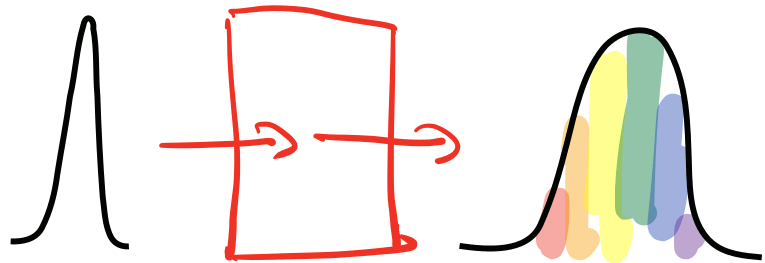
\includegraphics[width=0.5\textwidth]{./files/dispersion.svg.png}
    \end{flushright}
  \end{wrapfigure}

Une solution consiste à précompenser cette dispersion via des éléments optiques comme une suite de prismes ou de réseaux de diffraction positionnés en amont de l'injection \cite{fork_negative_1984}. Cette solution permet de réduire la largeur temporelle du pic en sortie de fibre, et donc de conserver l'effet deux photons. On rencontre un autre obstacle pour des impulsions de haute énergie. C'est l'automodulation de phase par effet Kerr \cite{agrawal_nonlinear_2000}. Cet effet est lié aux propriétés non linéaires du milieu traversé, qui change d'indice en fonction de l'intensité lumineuse qui le parcourt. Il en résulte également un élargissement de l'impulsion. Cet effet apparaît pour des puissances moyennes relativement faibles (10 mw \cite{helmchen_miniaturization_2013}), ce qui empêche d'utiliser des impulsions optimalement courtes (<1 ps \cite{helmchen_miniaturization_2013}) avec de telles fibres. Des techniques existent pour précompenser cette distorsion \cite{clark_fiber_2001} \cite{lefort_sub-30-fs_2014}, mais elles sont peu répandues car difficiles à mettre en place \cite{helmchen_miniaturization_2013}. De plus, ces problèmes peuvent être contournés par les fibres à âme vide.

\subsection{Fibre à âme vide}

Les phénomènes de dispersion et de non-linéarité sont dus à l'interaction avec la matière. Pour les contourner, il faut donc que les impulsions à haute énergie se propagent dans le vide. L'effet de réflexion totale sur le dioptre cœur/enveloppe ne peut plus être utilisé, car il faudrait un milieu d'indice plus petit que 1, c’est-à-dire dans lequel la lumière se propage plus vite que dans le vide, ce qui n'est pas possible. Intéressons-nous au guide d'ondes creux.

\subsubsection{Guide d'onde métallique ou diélectrique}

Une idée pour confiner la lumière dans un guide unidimensionnel est d'utiliser le phénomène de réflexion métallique, comme sur un miroir. En 1964, un article s'intéresse aux guides d'ondes dans le contexte des télécommunications optiques à longue distance \cite{marcatili_hollow_1964}. Les solutions qui semblaient les plus prometteuses à l'époque consistaient soit en une séquence de lentilles et de miroirs, soit en un tuyau métallique ou diélectrique. Le guide d'onde creux circulaire suscite un intérêt pour sa simplicité et sa bonne transmission sur de très longues distances, mais l'article montre que les pertes augmentent très rapidement avec la courbure de la trajectoire.

\subsubsection{Fibres à cristaux photoniques}

Une autre idée consiste à utiliser un phénomène de réflexion par interférences comme le miroir de Bragg. Un tel miroir est constitué d'une succession périodique de couches d'indice différents et permet d'obtenir une réflexion quasi totale à la longueur d'onde du motif. Différents modèles sont illustrés en figure \ref{FIGfiberexamples}.

\paragraph{Fibres à réseaux de tubes}
On trouve ce genre de réseau pour la première fois en 1999 sous forme de fibres à cristaux photoniques \cite{cregan_single-mode_1999} ou plus tard sous la forme de fibres microstructurées \cite{argyros_hollow-core_2006}. En 2010, Vincetti \emph{et al} montrent par analyse numérique que seule la première couche de tubes joue un rôle important dans les propriétés de ces fibres \cite{vincetti_waveguiding_2010}. Ce qui donne des fibres constituées d'un seul réseau de tube.

\paragraph{Fibres à motif Kagomé}
L'idée du réseau de diffraction a également donné lieu aux fibres à réseau trihexagonal, ou "Kagomé". De telles fibres ont été construites pour la première fois en 2002 sous le nom de fibre à cristaux photoniques. Le gain était alors de l'ordre de 2 dB/m \cite{benabid_stimulated_2002}. En 2011, un gain de 180 dB/km a été obtenu avec de telles fibres \cite{wang_low_2011}.
Cependant, en 2010, Février \emph{et al} montrent par analyse numérique que les propriétés de ces fibres ne reposent pas tant sur le motif périodique que sur la forme du cœur \cite{fevrier_understanding_2010}, ce qui ouvre la voie aux fibres à cœur hypocycloïde. 

% Un des problèmes des fibres à structure géométrique est la sensibilité aux déformations. Puisque le guidage est lié à la géométrie de la fibre, les déformations qui changent cette géométrie altèrent le guidage. Cela peut prendre la forme de perte de transmission, de couplage entre les modes, d'incidence sur la polarisation. Mais cette sensibilité aux déformations dépendant de la géométrie de la fibre, certaines configurations donnent des résultats très satisfaisants.

\subsubsection{Fibres à courbure négative}

Les idées de fibre à réseau de tubes unique et de fibres à cœur hypocycloïde se rejoignent dans un même concept : les fibres à courbures négatives. En 2016, Yu et Knight publient une revue sur l'histoire de ces fibres et leurs mécanismes \cite{yu_negative_2016}. Ils commentent entre autres l'atténuation, les bandes de transmission et les pertes de courbure \cite{belardi_effect_2013}. Ces critères rendent cette famille de fibres particulièrement adaptée à notre application. En effet, les larges bandes de transmission permettent de guider plusieurs longueurs d'onde, aussi bien pour l'imagerie un photon que deux photons, la faible atténuation permet de conserver la puissance du laser nécessaire à l'effet deux photons, et les faibles pertes de courbure permet de conserver une illumination stable pendant la rotation du microscope.

% IGN VolkerComment2
% You have to make the effort and write all this in your thesis. It is not sufficient to just refer to the review. Explain the light guidance mechanism, show figures, ... .



\subsection{Utilisation des fibres en microscopie embarquée}

% Dans un microscope statique, la source laser peut être guidée jusqu'à l'échantillon par des miroirs, mais dans un microscope mobile il faut soit embarquer la source laser directement sur le microscope, soit la guider de manière flexible quels que soient les mouvements. Dans le cas d'une source laser deux photons très volumineuse, il est impossible de l'embarquer, la solution adoptée est donc une fibre optique adaptée. De telles fibres optiques capables de guider un laser deux photons sont complexes à produire. Avant de nous intéresser aux microscopes à fibre couramment utilisés dans la recherche sur le rongeur, introduisons les caractéristiques d'un guide d'onde. 

Les propriétés de guidage de la lumière d'une fibre optique lui permettent d'alléger considérablement ou de déporter certaines parties des microscopes pour les rendre compatibles avec l'imagerie embarquée. Un microscope est en effet composé d'un axe d'illumination, d'un échantillon, et d'un axe de détection. Les axes peuvent être séparés dans différents bras ou réunis sur une portion du montage optique et sont généralement composés d'éléments optiques rigides passifs tels que des objectifs, miroirs, filtres... Ces différentes parties parfois très volumineuses peuvent être remplacées ou déportées à l'aide d'une fibre optique. Nous allons voir par la suite plusieurs types de microscopes embarqués utilisant une fibre optique.

\begin{figure}
\centering
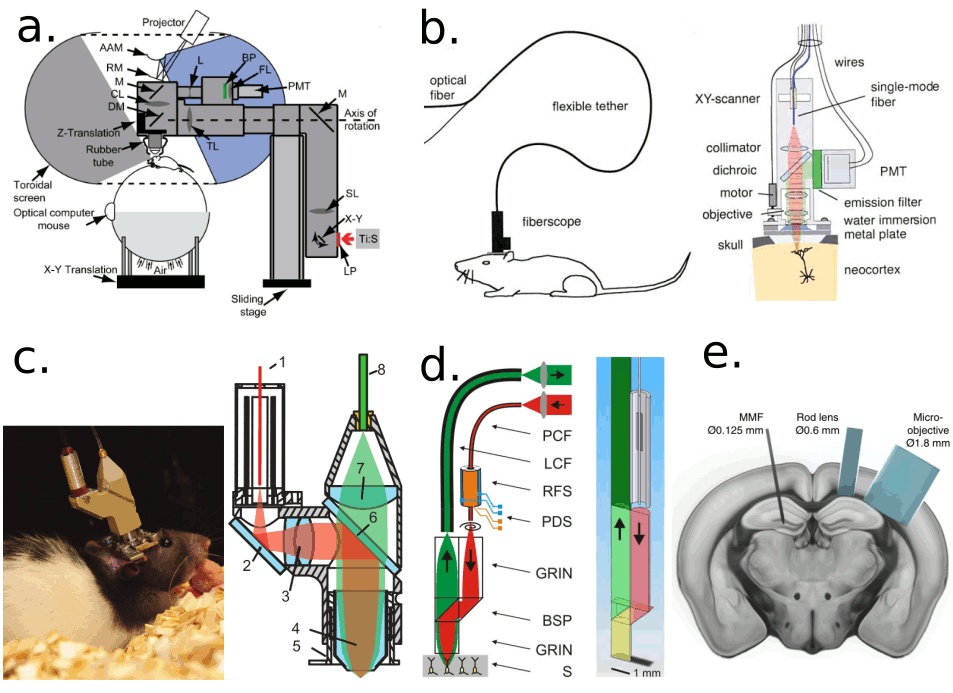
\includegraphics[width=\textwidth]{./files/fiber_functional_imaging.svg.png}
\caption{Différentes techniques de microscopie en imagerie neuronale fonctionnelle chez le rongeur.\\
a. Un microscope deux photons statique réalise l'imagerie du cerveau d'une souris lors d'une expérience en réalité virtuelle \cite{dombeck_functional_2010}.\\
b. Un microscope deux photons est fixé sur la boite crânienne d'un rat. Le laser est guidé à travers une fibre à cœur de verre dont la dispersion est précompensée. L'unité de détection est intégrée au microscope \cite{helmchen_miniature_2001}.\\
c. Un microscope deux photons est fixé sur le crane d'un rat, mais l'unité de détection est externe, la lumière étant collectée par une fibre \cite{sawinski_visually_2009}. \\
d. Un fibroscope deux photons utilise des fibres à gradient d'indice comme lentilles pour réduire l'encombrement. Le laser est guidé au moyen d'une fibre à cristaux photoniques et la lumière est collectée par une fibre à large cœur \cite{engelbrecht_ultra-compact_2008}. \\
e. Un endoscope sans optique permet de réduire considérablement l'encombrement et d'atteindre des régions plus profondes du cerveau, mais nécessite une calibration préalable \cite{turtaev_high-fidelity_2018}.
}
\end{figure}


% Functional imaging in freely moving animals (review)
% Advances in Light Microscopy for Neuroscience (review)

% 1P vs 2P
% Fiber optic in vivo imaging in the mammalian nervous system

\subsubsection{Imagerie sur rongeur à tête fixée}

Une méthode répandue en imagerie cérébrale sur rongeur est de fixer un animal sous un microscope classique immobile. Le cerveau est rendu accessible par une opération chirurgicale pendant laquelle la boîte crânienne est retirée localement et remplacée par une vitre. Le fait d'immobiliser la tête pendant l'imagerie peut limiter le répertoire comportemental et constituer une gêne pour l'animal. Une solution est un système où le rat se positionne volontairement sous le microscope \cite{scott_cellular_2013}, une autre est le système en réalité virtuelle. Dans cette deuxième solution, le rongeur marche sur une boule en polystyrène sur coussins d'air alors qu'un environnement visuel est projeté sur un écran autour de lui \cite{dombeck_functional_2010}. Le microscope est ici entièrement statique et rigide. La réalité virtuelle a également été utilisée avec des enregistrements en électrophysiologie \cite{aronov_engagement_2014}\cite{whitlock_navigating_2014}.

% IGN VolkerComment2
% You have to write all this from the point of view of the fiber application. Go straight to the challenge to record in freely moving animals and the development of portable fiber scopes ...


% \subsubsection{Microscope embarqué}
% An implantable and fully integrated complementary metal–oxide semiconductor device for in vivo neural imaging and electrical interfacing with the mouse hippocampus \cite{ng_implantable_2008}

\subsubsection{Déportation de l'illumination}

Une pièce particulièrement volumineuse dans les microscopes multiphotons utilisée pour l'imagerie neuronale est le laser pulsé. En effet, ces systèmes dépendent de beaucoup d'éléments optiques et d'une stabilité thermique et mécanique poussée. Pour construire des microscopes embarqués, il est donc nécessaire de guider le laser depuis la source jusqu'à l'échantillon, ce qui est réalisé à l'aide de fibre optique. Il est possible d'utiliser une fibre optique monomode à cœur de verre \cite{helmchen_miniature_2001} \cite{sawinski_visually_2009} \cite{zong_fast_2017} à condition de précompenser la dispersion pour conserver une impulsion suffisamment courte pour produire l'effet non linéaire recherché, ce qui est réalisé avec une paire de réseaux de diffraction. Une alternative est d'utiliser une fibre à cœur creux \cite{tai_two-photon_2004} \cite{choi_improving_2014} \cite{piyawattanametha_vivo_2009} \cite{klioutchnikov_three-photon_2020}.
La partie de détection est quant à elle également embarquée. On peut avoir un simple photomultiplicateur/photodiode pour l'imagerie par balayage \cite{helmchen_miniature_2001} ou un capteur CMOS pour une imagerie en champ plein \cite{scott_imaging_2018}.

\subsubsection{Déportation de l'illumination et de la détection}

Dans les exemples précédents, le laser est amené par une fibre, mais le capteur est sur place, le signal repartant sous forme de signal électrique. Il est également possible de déporter le système de détection en collectant la lumière par fibre optique. Certains utilisent pour cela une fibre multimode \cite{piyawattanametha_vivo_2009} \cite{sawinski_visually_2009}, d'autres une \emph{fibre plastique} \cite{klioutchnikov_three-photon_2020}, d'autres encore un faisceau de fibres \cite{zong_fast_2017}. Dans ce cas, la lumière collectée est mesurée en sortie de fibre à l'aide d'un système optique adapté sans limite d'encombrement. On peut ainsi utiliser des systèmes volumineux et sensibles aux vibrations comme des sources laser régulés en température ou des circuits de détection munis d'une électronique complexe.

\subsubsection{Lentilles à gradient d'indice}

Malgré la déportation de l'illumination et de la détection, les systèmes optiques restent encore assez volumineux du fait des composants utilisés et des éléments mécaniques nécessaires. Une possibilité pour pousser la miniaturisation encore plus loin est d'utiliser des fibres à gradient d'indice (\emph{GRIN lens, GRadient INdex lens}). Ces fibres sont constituées d'un milieu à gradient d'indice qui leur donne des propriétés similaires à des lentilles mais sont plus fines et ne nécessitent pas d'éléments mécaniques. Cela permet d'obtenir des microscopes ultra-compacts portables et de poids très réduit \cite{flusberg_vivo_2005}\cite{engelbrecht_ultra-compact_2008}.

\subsubsection{Microendoscopes}

% IGN VolkerComment2
% Why do you describe this. Where is the link to your work? You can use this in the discussion and propose that your fiber can be also used to collect the fluorescent light. With the small mode field diameter this would create a confocal like configuration.

D'autres techniques d'imagerie neuronale se passent même d'optique et sont uniquement constitués d'une fibre insérée dans l'échantillon. On parle alors plutôt de microendoscope. L'idée générale est d'utiliser la même fibre pour éclairer l'échantillon et collecter la lumière. Des éléments actifs peuvent être utilisés pour moduler le front d'onde, et plusieurs techniques reposent sur une phase de calibration préalable \cite{papadopoulos_high-resolution_2013}\cite{ohayon_minimally_2018}\cite{turtaev_high-fidelity_2018}. Ces techniques utilisent des fibres optiques multimodes classiques. L'avantage de l'endoscopie est que les tissus sont traversés par la fibre, et pas directement par la lumière, ce qui contourne le phénomène de dispersion. Il existe également des systèmes plus sophistiqués qui combinent plusieurs fibres en une seule de manière à profiter de propriétés différentes pour l'émission et collection de lumière \cite{andresen_two-photon_2013}\cite{kudlinski_double_2020}\cite{lombardini_high-resolution_2018}.



\section{Caractérisation et utilisation de fibres à âme vide}

Nous avons vu dans la partie précédente qu'une fibre optique permet de guider la lumière, que ce soit pour éclairer l'échantillon ou collecter le signal. Les fibres de verre conviennent bien aux applications classiques, mais posent des problèmes d'interaction lumière-matière lors de la transmission d'impulsions à haute énergie pour la microscopie multiphoton et nécessitent une précompensation de la dispersion. Les fibres à âme vide permettent de contourner ces problèmes et ont déjà été largement utilisées dans des microscopes embarqués sur rongeur \cite{tai_two-photon_2004} \cite{flusberg_vivo_2005} \cite{engelbrecht_ultra-compact_2008} \cite{piyawattanametha_vivo_2009} \cite{choi_improving_2014} \cite{klioutchnikov_three-photon_2020}. C'est donc vers celles-ci que nous nous sommes tournés. Aucune fibre disponible commercialement ne permettait de transmettre à 930 nm, nous avons donc testé plusieurs modèles de recherche et développement de l'entreprise \href{http://www.glophotonics.fr/}{Glophotonics} (Fig. \ref{FIGfibercomparison}).

% IGN VolkerComment2
% What are our requirements ? Detail this ...

\subsection{Comparaison de fibres}

% OK Volker (GLO all fibers)
% In collaboration with GLO we tested several different fiber types. Go through all of them ! Show the image of the cross section of this fiber and give all details of the fiber geometry: core diameter, total diameter, number of cladding tubes, tube wall thickness, cladding tube diameter, NA, mode field diameter (1/e2), curvature parameter (For b definition, see Opt. Exp. 21, no. 23, 28597, 2013)... .

% OK VolkerComment2
% No, we did not record with these fibers. The mode field diameter was to large and the instabilities to bending were to large. Or do you have successful recordings with these fibers? The Brighton experiments were done with the fiber PMC-C-1C-R&D2

Au début, nous avons utilisé des fibres Kagome ayant une bande de transmission dans l'infrarouge. Ces fibres ont permis de réaliser les premiers enregistrements deux photons de l'activité neuronale mais sont sensibles aux déformations, ce qui empêche l'enregistrement lors de la rotation du microscope. Ensuite, nous avons cherché à permettre à la fois la transmission d'un laser 1P et 2P, d'où l'utilisation de fibres avec plusieurs bandes de transmission. Parmi ces fibres, nous avons retenu le modèle PMC-C-9005 B2 qui permet une bonne transmission (97\% à 930 nm sur 1,5 m de fibre contre 70\% pour PMC-C-1C-R\&D2) (Fig. \ref{FIGfibercomparison}). J'utilise ce modèle comme référence par la suite.

\begin{figure}
    \centering
    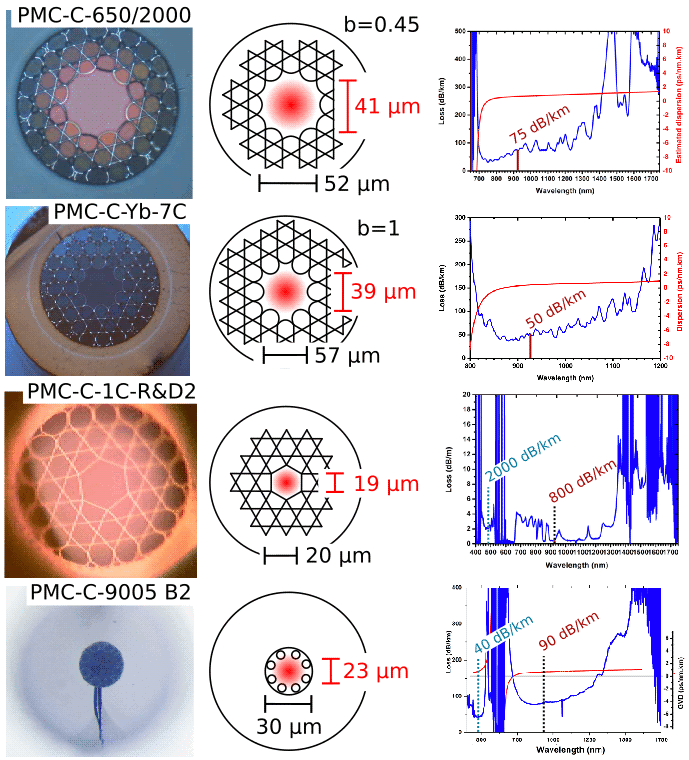
\includegraphics[width=\textwidth]{./files/glofibers.svg.png}
    \caption{Comparaison de plusieurs fibres fournies par Glophotonics. Les schémas représentent la largeur du cœur (en noir) et la largeur du mode propre (en rouge). Dans le spectre de transmission, on s'intéresse à la valeur à 930 nm et à 488 nm si possible. La valeur de la dispersion est toujours la même, environ à 1 ps/nm.km. Les trois premières fibres ont un motif de Kagomé, alors que la dernière n'est composée que d'une couche de capillaires. Seule la troisième fibre a un cœur hexagonal, les autres ont un cœur hypocycloïde. La valeur du paramètre de courbure est notée b, comme défini dans Debord \emph{et al} \cite{debord_hypocycloid-shaped_2013}.
    \label{FIGfibercomparison}}
    \end{figure}

% La figure \ref{FIGfibercomparison} compare plusieurs modèles de fibre. Les deux premières ont une large bande de transmission dans l'infrarouge et un mode propre large. Les autres ont deux bandes de transmission qui couvrent à la fois le bleu et l'infrarouge

\subsection{Injection d'un laser dans une fibre}

% OK Volker Add a motivation (for 1P)

Une fibre capable de guider à la fois un laser 1P et un laser 2P permettrait de réaliser l'acquisition du cerveau en changeant facilement la longueur d'onde d'excitation et de mettre en évidence les différences dans l'activité neuronale causées par l'environnement visuel. Un autre avantage non négligeable est de faciliter l'alignement du système optique et de l'échantillon, plus difficile en lumière infrarouge. Je décris ici le processus d'injection dans une fibre et le montage que j'ai mis en place pour passer du laser 1P au laser 2P à l'aide d'un miroir amovible. 

\subsubsection{Principe}

Pour injecter le laser dans la fibre, il faut aligner tous les éléments dans l'axe optique et régler finement les degrés de liberté en translation et en rotation. De plus, comme on souhaite un couplage monomode, il faut faire coïncider le mode laser d'entrée de fibre avec le mode propre de la fibre. Le laser ayant une largeur initiale de D, il faut le ramener à une largeur $w$ égale au mode propre de la fibre (23 µm ± 1 µm d'après la documentation). Pour cela, il faut utiliser une lentille de focale f et satisfaire l'équation suivante :

$$
f = D\frac{\pi w}{4\lambda}
$$

\subsubsection{Injection 2P}

Le laser \emph{Mai-Tai} que j'ai utilisé délivre un faisceau quasiment gaussien (M²<1.1) et son waist ($w_0$) est large d'environ 1 mm. Ces valeurs sont données par la documentation pour une utilisation à 800 nm, mais elles peuvent évoluer légèrement en accordant la longueur d'onde de fonctionnement. La largeur d'un faisceau gaussien au long de sa propagation ($z$) est définie par :

$$
w(z) = w_0 \, \sqrt{ 1+ {\left( \frac{z}{z_\mathrm{R}} \right)}^2 } \qquad \text{avec} \qquad
z_\mathrm{R} = \frac{\pi w_0^2 }{\lambda}
$$

Le diamètre du laser est donc d'environ 2 mm après un mètre de propagation. En prenant D = 2 mm, $\omega$ = 23 µm, et à $\lambda$ = 915 nm, on trouve donc f = 40 mm, c'est pourquoi j'ai utilisé une lentille de focale 40 mm (référence Thorlabs AC254-040-B-ML). Cette lentille dispose également d'un traitement de surface pour optimiser la transmission dans l'infrarouge.

% IGN Volker (fig alignment)
% show a photo of this configuration and explain the alignment procedure with a schema
% Give the damaging threshold of the fiber as a reference -> I do not know

J'ai fixé une extrémité de la fibre sur une platine de translation $xyz$ à 40 mm de la lentille (Fig. \ref{FIGinjectiongraystack}). Pour faciliter l'alignement, j'ai tout d'abord injecté un laser visible grâce à un connecteur fibre à fibre dans l'autre extrémité. Cela m'a permis de pré-aligner deux miroirs sur support rotatifs en visant l'orifice du laser parallèlement à l'axe optique. En allumant le laser à faible puissance pour ne pas endommager la fibre, on obtient alors facilement une transmission suffisante pour pouvoir mesurer la puissance en sortie de fibre. À partir de cette étape, il suffit d'optimiser la puissance transmise en jouant sur les réglages. Dans un premier temps, les deux degrés de rotations de chacun des deux miroirs, et dans un deuxième temps, les deux degrés de rotation du second miroir et les trois degrés de translation de la platine. Cette technique permet d'obtenir en un temps raisonnable ($\sim$1h) une transmission optimale ($\sim$96\%).

\subsubsection{Injection combinée 2P + 1P}

\begin{figure}
    \centering
    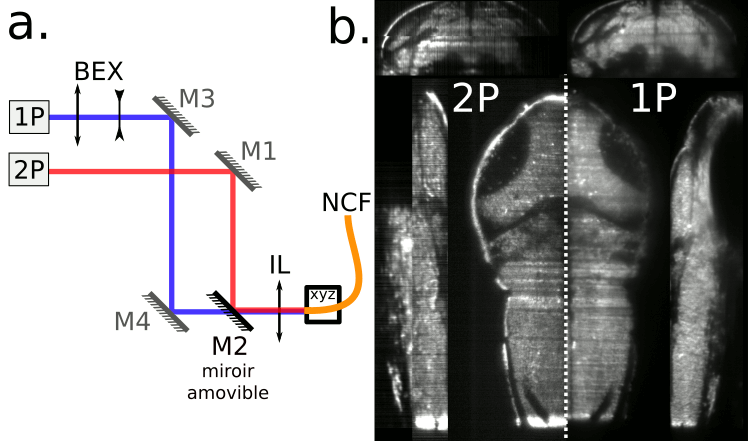
\includegraphics[width=\textwidth]{./files/injection+graystack_1P2P.svg.png}
    \caption{Injection des deux lasers dans la fibre et images ainsi obtenues.
    \\a. Pour aligner la source 1P et 2P, on injecte dans un premier temps un laser visible par l'autre extrémité de la fibre et l'on joue sur les miroirs M1 et M2 pour pointer vers la sortie du laser 2P. Une fois les miroirs préalignés, on règle le laser 2P et on optimise la puissance en sortie de la fibre avec les miroirs M1 et M2 et la platine xyz. Ensuite, on escamote le miroir M2 pour aligner le laser 1P avec les miroirs M3 et M4 sans toucher à la platine xyz. Le miroir M2 est amovible et permet de basculer entre l'injection 1P et 2P. (BEX = \emph{Beam Expander}, IL = \emph{Injection Lens}, NCF = \emph{Negative Curvature Fiber})
    \\ b. Comparaison entre un volume statique imagé en deux photons (2P) et en un photon (1P). Le volume deux photons est imagé en deux parties pour éviter d’illuminer les yeux (on voit nettement l’ombre de l'œil sur la coupe sagittale en un photon). Le pas est de 1 μm par couche. Le temps d'exposition est de 10 ms dans les deux cas.
    \label{FIGinjectiongraystack}}
    \end{figure}

Pour injecter un deuxième laser, il faut à nouveau faire coïncider le mode de la fibre avec celui du laser, mais en conservant la même lentille d'injection et sans utiliser la platine de translation (Fig. \ref{FIGinjectiongraystack}). Il faut donc adapter la largeur du faisceau à l'aide d'un télescope ou \emph{beam expander} (BEX). En remplaçant 915 nm par 488 nm, on obtient D = 1 mm. La lentille étant optimisée pour l'infrarouge, sa transmission dans le bleu n'est que de 50\%, mais la puissance du laser bleu est suffisante pour compenser cette perte. Par contre, la fibre n'est pas tout à fait monomode à cette longueur d'onde, et l'on distingue clairement en sortie le mode TEM11 ou les modes TEM10 / TEM01 en fonction de la position de la fibre. La meilleure transmission obtenue est de l'ordre de 50\%, mais cela est suffisant pour l'imagerie statique (fibre immobile).

On voit ainsi en figure \ref{FIGinjectiongraystack} (b.) la comparaison d'un même cerveau imagé en un photon et en deux photons. Il y a un léger décalage entre les deux images qui peut être lié à une aberration chromatique des objectifs du module de balayage et à l'interface air-eau lors de l'entrée dans la cuve et les volumes ne sont donc pas tout à fait superposables.


\subsection{Propriétés}

% IGN introduire

\subsubsection{Dispersion et pré-compensation}

Un paramètre important pour la transmission d'un laser pulsé est la dispersion. C'est celui qui nous force à utiliser des fibres à cœur creux et qui permet de conserver une impulsion aussi courte que possible. Mais la dispersion d'une fibre à cœur creux n'est pas nulle, elle est de l'ordre de 1 ps/nm/km (élargissement temporel / largeur spectrale / distance parcourue) comme on peut le voir sur la courbe. La largeur spectrale d'une impulsion vaut 28 nm, elle est donnée par la formule :

$$
\Delta \lambda_t = \frac{\lambda^2}{c\Delta t}
$$

Pour une impulsion de 100 fs à 915 nm, cela donne un élargissement de l'ordre de 28 fs au bout d'un mètre de propagation dans la fibre, soit une perte de concentration de 30\% et donc une perte d'effet deux photons de 50\%. Heureusement, il est possible de pré-compenser cette dispersion à l'aide d'un système optique placé en amont de la fibre. Le laser \emph{Mai-Tai} est justement accompagné d'un élément \emph{Deepsee} qui permet une telle précompensation réglable de -8 900 à -24 500 fs² d'après la documentation.

% (citation documentation)
% > The amount of dispersion, or GVD compensation, provided for each wavelength depends on the position of the DeepSee motor that moves optical material on a stage within the beam path.

En mesurant la durée de l'impulsion en sortie de fibre à l'aide d'un autocorrélateur, on confirme que la précompensation permet de retrouver une impulsion de 100 fs dans l'échantillon.

\subsubsection{Pertes de courbure}

% OK Volker show the data and give all fiber details (fiber bending loss)
% IGN Volker (kagome bending loss)
% This is true for the hypocycloid fibers but does not apply to my knowledge to the Kagome fiber lattice that you discussed just before. Explain why there is a dependence of the gain on curvature. And explain the waveguidance mechanism in the hypocycloid fibers (anitresonance effect ... )

Les propriétés de transmission de la fibre peuvent varier avec la courbure de celle-ci. La transmission est généralement optimale pour une fibre droite et se détériore suivant le rayon de courbure avec des pertes mesurées en dB. Une fibre PCNC-FC-K13-001 que je ne présente pas ici donnait des variations de transmission de l'ordre de 20\% pour un rayon de courbure de 5 cm.
Lors d'une expérience, la rotation du microscope engendre des déformations de la fibre, et donc des variations de transmission. L'éclairage incident se retrouve corrélé à la stimulation, ce qui crée un signal parasite. Un signal parasite supérieur à 1\% détériore trop le rapport signal à bruit et empêche l'analyse des données. On cherche donc à caractériser les pertes de transmission liées à la courbure. Pour cela, il suffit de placer un puissance-mètre en sortie de fibre et de faire varier la courbure.

Pour tester les propriétés de la fibre en fonction de sa courbure, j'ai mesuré l'intensité et la polarisation du faisceau en sortie pour une polarisation linéaire et circulaire en entrée. Des modèles numériques \cite{yu_negative_2016} \cite{setti_flexible_2013} \cite{frosz_analytical_2017} suggèrent que le gain évolue de manière inversement proportionnelle au carré du rayon de courbure. Cette relation est également observée sur notre fibre (Fig. \ref{FIGfibercarac}). Les pertes par mètre de fibre courbée restent cependant petites même pour un rayon assez court. Elles valent 0.1 dB ($\sim$2\%) pour un rayon de courbure de 7 cm (Fig. \ref{FIGfibercarac}). Je n'ai trouvé aucun modèle pour la polarisation, mais les expériences montrent que pour une polarisation linéaire en entrée, une courbure de la fibre engendre une rotation de la polarisation en sortie. Pour une polarisation circulaire en entrée, invariante par rotation, on détecte un léger changement d'ellipticité en sortie.

En conditions réelles, on peut s'arranger pour limiter la courbure et répartir les déformations sur l'ensemble de la fibre. Par exemple, la fibre peut être attachée à une tige de rigidité plus élevée. On peut alors facilement interdire un rayon de courbure inférieur à 20 cm sur un mètre de fibre et donc limiter les pertes associées à 0.01 dB, soit 0.2\%.

% OK Volker (fiber curvature real conditions)
% pourqui c'est le pire des cas ? Dans quelle context? I do not understand your argument. What is the range of curvature change in your experimental configuration?

\begin{figure}
    \centering
    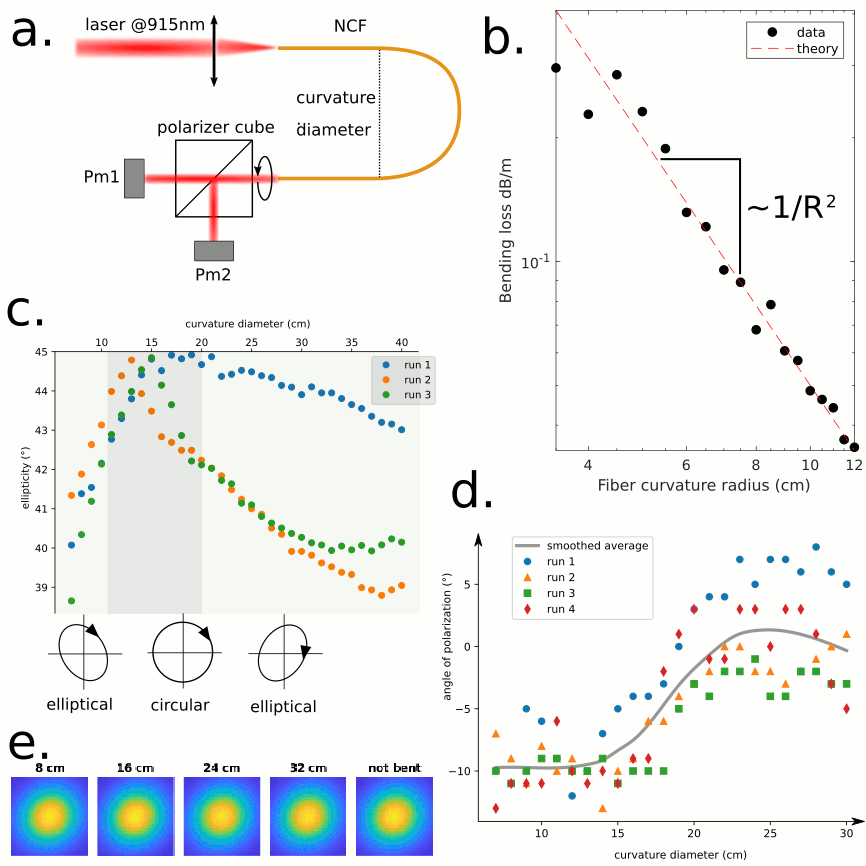
\includegraphics[width=0.75\textwidth]{./files/fiber_bending.svg.png}
    \caption{Propriétés de la fibre en réponse à une courbure en demi arc de cercle (gain et polarisation).
    \\ a. La fibre est courbée sur un demi arc de cercle avec un rayon de courbure variable. Les puissance-mètres Pm1 et Pm2 mesurent l'intensité sur les deux bras de polarisation en sortie d'un cube monté sur un goniomètre. 
    \\ b. Pertes en sortie de fibre exprimé en dB par mètre de fibre courbée en fonction du rayon de courbure.
    \\ c. Profil d'intensité en sortie de fibre pour différentes courbures (non affecté).
    \\ d. Pour une polarisation quasi circulaire, variation de l'ellipticité en fonction du diamètre de courbure.
    \\ e. Pour une polarisation quasi linéaire, variation de l'angle de polarisation en fonction du diamètre de courbure.
    \label{FIGfibercarac}}
    \end{figure}

% IGN VolkerComment2
% You have to write the figure legend ! You have to describe every panel and give the meaning of the appreciations.

% OK Volker output profile
% (via rocketchat) Add also the measurement of the fiber output profile as a function of bending diameter to your thesis. Your measurement shows that at 915nm the profile does and thus the mode does not change. 

\subsubsection{Polarisation}
% OK Volker (context for polarization -> de Vito)
% You start this paragraph totally out of context. So far you talked about the fiber properties. Here you talk about detected signal in the light sheet configuration. You have to introduce this properly and develop the transition.

On voit dans la section précédente que la courbure a un effet sur la transmission négligeable dans le contexte de l'imagerie. Cependant, un autre aspect peut influencer la quantité de lumière détectée : la polarisation. La sensibilité d'un milieu fluorescent aux variations de polarisation dépend de la polarisation (rectiligne, circulaire, orientation), de la configuration d'éclairage (parallèle ou orthogonale, Fig. \ref{FIGpolarisation}), du type d'absorption (un ou deux photons).

\begin{figure}[h!]
    \centering
    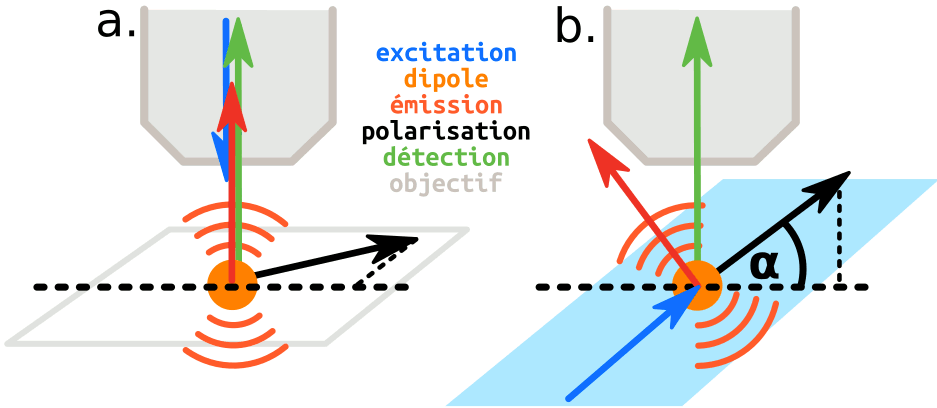
\includegraphics[width=0.75\textwidth]{./files/polarization_plane.svg.png}
    \caption{Comparaison d'un microscope classique et d'un microscope à feuille de lumière du point de vue de la polarisation.
    \\ a. Dans un microscope classique, l'axe optique d'excitation et de détection sont verticales, et la polarisation est dans le plan orthogonal. La lumière détectée ne dépend donc pas de la direction de polarisation (sauf si les fluorophores sont orientés).
    \\ b. Dans un microscope à feuille de lumière, l'onde d'excitation se propage dans un plan horizontal, orthogonal à l'axe de détection. La polarisation est dans un plan vertical. On note $\alpha$ l'angle entre la polarisation et le plan horizontal. Pour $\alpha$ = 0°, la lumière détectée est maximale, pour $\alpha$ = 90°, elle est minimale (sauf si les fluorophores sont orientés).
    \label{FIGpolarisation}}
\end{figure}

\paragraph{Direction du fluorophore}

Un fluorophore peut être modélisé par un dipôle électrostatique. La fluorescence peut alors être décrite comme la succession d'un phénomène d'absorption de l'onde incidente et d'un phénomène de ré-émission selon les lois du rayonnement dipolaire électrique. Ce phénomène est anisotrope et dépend de la polarisation incidente et du moment dipolaire. Dans un milieu fluorescent isotrope, la fluorescence est en majorité due aux fluorophores correctement orientés, ce qu'on appelle la photosélection. Par exemple, pour une polarisation rectiligne horizontale, les fluorophores dont le moment dipolaire est horizontal sont responsables de la majorité de la fluorescence.

% citer Weber rotational 1953
% fluorophores soumis à un mouvement Brownien

\paragraph{Direction d'excitation}

Quand l'axe d'excitation est parallèle à l'axe d'observation (par exemple en microscopie confocale ou deux photons classique), le plan de polarisation est orthogonal aux deux, un photon absorbé est donc réémis dans la même direction quelle que soit la polarisation (Fig. \ref{FIGpolarisation} a.). Au contraire, quand l'axe d'excitation est orthogonal à l'axe d'observation (par exemple en microscopie à feuille de lumière), l'angle de polarisation influe sur la direction d'émission (Fig. \ref{FIGpolarisation} b.). Pour une polarisation rectiligne orthogonale à l'axe d'observation ($\alpha$=0°), on se retrouve dans un cas similaire au précédent, mais pour une polarisation rectiligne colinéaire à l'axe d'observation ($\alpha$=90°), on obtient une diminution du signal de fluorescence dans l'axe d'observation.
On confirme ceci à l'aide d'une lame $\lambda$/2. En tournant une polarisation rectiligne et en observant la fluorescence du cerveau, on passe d'une intensité détectée maximale à une intensité minimale. Pour une polarisation circulaire, on obtient une valeur intermédiaire.


% IGN faire des calculs compliqués pour remplacer ces calculs faux
% Cette valeur de l'intensité minimale s'explique ainsi : pour une polarisation orthogonale à l'axe d'observation ($\alpha$=90°), un dipôle faisant un angle $\theta$ avec la polarisation (et donc $\frac{\pi}{2}-\theta$ avec la détection) est excité proportionnellement à $\cos\theta$ et détecté proportionnellement à $\cos(\frac{\pi}{2}-\theta) = \sin\theta$. Pour une répartition égale des dipôles pour tout ange $\theta$, la fluorescence détectée est donc de :
% $$
% \int_0^\frac{\pi}{2} \sin(\theta)\cos(\theta) \mathrm{d}\theta = \left[ \frac{1}{2}\sin^2(\theta) \right]_0^\frac{\pi}{2} = \frac{1}{2}
% $$


% OK VolkerComment2
% Work over the figure legend. Each panel needs a to be introduced in the legend with a subtitle. The blue arrow indicates the excitation and not the emission.

\paragraph{Absorption deux photons}

En excitation deux photons, l'état de polarisation influe sur l'efficacité d'absorption. Un faisceau polarisé linéairement a un taux d'absorption deux photons plus élevé qu'un faisceau polarisé circulairement. Cependant, un faisceau polarisé circulairement conduit à une excitation plus homogène du fluorophore par photosélection. Le résultat est qu'une polarisation circulaire conduit à un signal détecté deux fois plus faible qu'une polarisation linéaire optimale, et de l'ordre d'une polarisation linéaire à 90° \cite{de_vito_effects_2020}. Idéalement, la polarisation en sortie de fibre doit donc rester linéaire et horizontale quelle que soit sa déformation. J'ai donc cherché à caractériser les modifications de polarisation induites par une déformation de la fibre.

% IGN faire les mêmes calculs compliqués mais avec ^4 au lieu de ^2

\paragraph{Caractérisation des effets sur la polarisation}

Une déformation de la fibre peut entrainer deux modifications sur la polarisation : une rotation et un changement d'ellipticité. Pour les mesurer, j'ai placé un cube polariseur en sortie de fibre équipé d'un puissance-mètre sur chaque bras. Pour chaque position de la fibre, j'ai tourné le cube de manière à minimiser la puissance mesurée sur un bras (et donc maximiser la puissance sur l'autre bras). Cela permet de déduire l'orientation de la polarisation (angle du cube) et son ellipticité (valeur du grand axe et petit axe). L'ellipticité ($\theta$) est définie par $\tan(\theta)=\frac{b}{a}$ où (a) est le grand axe et (b) le petit axe de l'ellipse. J'ai positionné la fibre en forme de U et ai réalisé des mesures pour des diamètres de courbure allant de 5 cm à 40 cm (Fig. \ref{FIGfibercarac}).

\paragraph{Rotation de la polarisation}

J'ai montré que la polarisation tournait significativement en fonction de la courbure de la fibre. Par exemple, entre un rayon de courbure de 15 cm et 25 cm, une polarisation linéaire peut tourner de 10° (variation du signal de $\sim$5\%). Ces valeurs de courbure sont celles qu'on peut attendre dans de bonnes conditions expérimentales, c'est pourquoi j'ai cherché à obtenir une polarisation invariante par rotation, c'est-à-dire une polarisation circulaire.

% OK Volker (real condition curvature)
% Again what is the expected curvature variation in your experimental configuration. What is the expected signal variation.

\paragraph{Changement d'ellipticité}

En polarisation circulaire ($\theta$ = 45°), la rotation n'est plus un problème, mais la fibre peut toujours transformer la polarisation circulaire en une polarisation elliptique, qui perd sa symétrie et devient donc sensible à la rotation. J'ai caractérisé la variation d'ellipticité dans le cas d'une polarisation circulaire. Les plus grandes variations d'ellipticité enregistrées sont de l'ordre de 5°. Pour vérifier comment ces différents éléments entrent en jeu, j'ai réalisé des tests en conditions réelles.

\begin{figure}
    \centering
    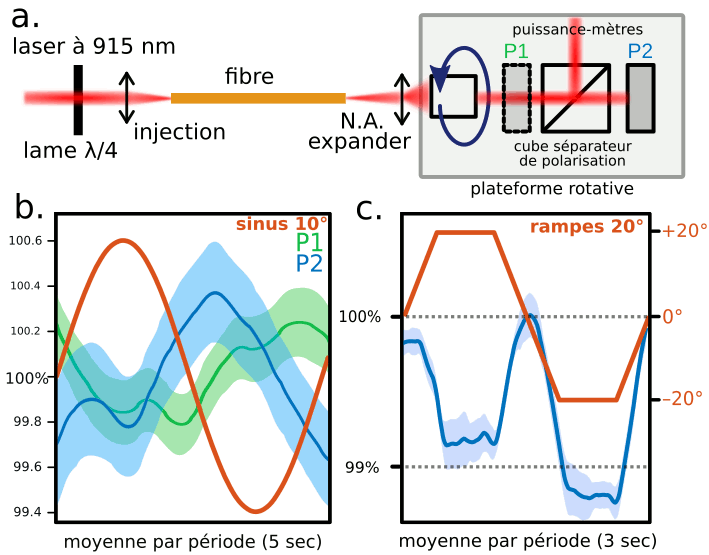
\includegraphics[width=0.75\textwidth]{./files/real-condition_intensity-variation.svg.png}
    \caption{Test de la fibre en conditions expérimentales. La variation de l'intensité détectée est une combinaison des pertes de courbure, du changement d'ellipticité et de la rotation de la polarisation. 
    \\ a. Montage expérimental pour test en conditions réelles. Un puissance-mètre peut être installé en position P1 (intensité seulement) ou P2 (intensité après cube séparateur de polarisation).
    \\ b. Réponse à une stimulation sinusoïdale périodique de 10°. On constate que les variations de puissance ne dépassent pas 0.6\% et que ces variations combinées aux changements de la polarisation (ellipticité et rotation) n'excèdent pas 1.2\%.
    \\ c. Réponse à une stimulation périodique en marches de 20°. Les variations combinées n'excèdent pas 1.2\%. On remarque que l'intensité maximale est atteinte pour un angle du moteur de 0°, soit la position de repos de la fibre.
    \label{FIGrealconditionsfiber}}
    \end{figure}

% IGN VolkerComment2
% You have to introduce the NA expander and show a schematic of the experiment

\subsubsection{Test avec rotation du microscope}

Après cette caractérisation statique de la fibre, j'ai testé comment les différents effets se combinent entre eux lors des déformations de la fibre attendues en conditions expérimentales. En retirant le deuxième objectif du module de feuille de lumière pour garder un faisceau collimaté, j'ai monté un cube polariseur et un puissance-mètre à la place de l'échantillon. À l'aide du moteur, j'ai soumis l'ensemble à des stimulations périodiques sinusoïdales et en rampe et j'ai mesuré les variations d'intensité pure, et les variations d'intensité après polariseur (Fig. \ref{FIGrealconditionsfiber}).

Finalement, les effets combinés des pertes de courbure, de la rotation de la polarisation et du changement d'ellipticité, engendrent des variations de l'intensité après polariseur inférieures à 1.2\% de la valeur au repos pour des déformations de la fibre atteintes en conditions expérimentales. Les effets parasites existent donc, mais ils sont connus et mineurs. Ils constituent une source de bruit d'amplitude connue, ce qui permet de les prendre en compte lors de l'analyse des données.

% IGN Volker (intensity change due to polarization)
% You have also to add the measured intensity change in the case if you would work with linear polarized light. In addition you have to make a measurement with GFP fish to see how much the real collected fluorescence depends on polarization and ellipticity.


\section{Effet de lentille thermique}\label{sectionthermallenseffect}

% OK VolkerComment (introduce thermal lens effect)
% You need to introduce better this part. In the previous sections you characterized hollow core fibers and identified a fiber that fulfills the stringent requirements to build a fiber coupled 2P-RLS. You should finish this part with the demonstration of successful 2P whole-brain imaging with single cell resolution in static mode. Then you discuss the next challenge to record during dynamic microscope rotation. The challenge arises as you observed large intensity fluctuations during microscope rotation that are independent of fiber properties. Then you discuss that this instability is related to water movements as you can induce it by moving the water in the chamber while keeping the microscope static. You discovered that this instability results from a thermal lens effect ....
% [rephrased]
% - demonstrate static 2P fiber coupled imaging
% - then discuss the dynamic mode challenges

On a vu que la fibre avait de bonnes propriétés en conditions réelles, pourtant en essayant d'imager un poisson en deux photons tout en bougeant le microscope, on observe des fluctuations d'intensité de grande amplitude (Fig. \ref{FIGwaterinstability}). En regardant attentivement à l'œil, on s'aperçoit que ces fluctuations sont liées à un déplacement de la zone la plus lumineuse le long de la direction de propagation du faisceau qui rend toute exploitation des données impossible. Cette observation a pu être expliquée par l'effet de lentille thermique (\emph{thermal lens effect}) modulé par un déplacement des masses d'eau de températures différentes.

% IGN VolkerComment2
% You have to describe in detail all the observations that led to the hypothesis that the thermal lens effect is the reason for the instability. 1. The instability increased with rotation frequency. At 0.01Hz sinusoidal stimulation at 10degree amplitude we had stable calcium imaging recordings. This showed that it is a dynamic effect. We hypothesized that the instability is related to water movements. You made two controls to demonstrate this: 1. Under static microscope conditions you could introduce laser focus movements by moving the water in the tank. 2. Recordings in agarose were stable. Show these results. Next, you made the observation that once opening the two-photon laser shutter that the light-sheet waist moves relative to its initial position by ~100μm along the laser axis. It takes several hundred of milliseconds before the laser focus equilibrates to a stable position. Show the corresponding kymographs. You hypothesized that the high-power infrared laser is absorbed by the water and modifies the refractive index of water along the laser path by local heating which changes the effective focal distance of the illumination objective. Once all temperature gradients are equilibrated the effective focal distance is stable. Rotating the microscope leads to water movements in the experimental chamber relative to the optical system due to inertia effects. Cold water comes into the laser path and changes transiently the effective focal distance. This mixing effect and thus the imaging artefact increases with increasing microscope acceleration. To test this hypothesis you performed (1) experiments in agarose to immobilize the water. Under these conditions no artifact was observed (show the data!). (2) You calculated the effect and compared your measurements with the theoretical description ... . Next you explain that initially you thought that the focal shift is caused mainly by the laser heating in the focus. Interestingly, the calculations show that every element along the laser path contribute equally to the focal shift. Show the calculation, plot a figure that demonstrates this effect and give an intuitive explanation. Now you can discuss the solutions to the problem: 1) You solution with the shutter 2) Reducing the laser path through the water!

Lorsqu'un faisceau traverse un milieu absorbant, ce milieu chauffe sur la trajectoire du faisceau, ce qui change son indice optique. Le gradient d'indice ainsi formé dévie les rayons, formant une lentille à gradient d'indice (GRIN lens). Pour l'eau, à 915 nm, le changement d'indice est de l'ordre de $-10^{-4}$ par degré. La température étant plus élevée au centre du faisceau, l'indice optique est plus faible, et donc la lentille équivalente est divergente. Cet effet peut être utile, par exemple pour mesurer le coefficient d'absorption d'un liquide \cite{whinnery_laser_1974}, mais il a deux conséquences gênantes dans mon cas. D'une part un effet statique lié à la perte de focalisation du faisceau altère l'effet deux-photons, d'autre part un effet dynamique lié à la réponse du système à une perturbation de la température d'équilibre dévie le faisceau lors des mouvements du microscope.

% IGN VolkerComment2
% (température plus élevée au centre du faisceau) Make a nice schematic to illustrate what you describe here
% (conséquences gênantes) Incomprehensible ... . Explain this more in detail.

\begin{figure}
    \centering
    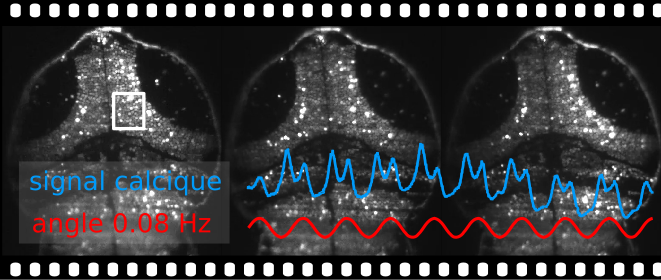
\includegraphics[width=0.85\textwidth]{./files/water_instability.svg.png}
    \caption{Images extraites d'un film montrant les changements d'intensité liés à l'effet thermique. On y voit la distribution d'intensité lumineuse se déplacer de gauche à droite (direction de propagation du faisceau) au rythme des mouvements du moteur. La plateforme est tournée suivant un mouvement sinusoïdal d'amplitude 10° à 0.08 Hz (en rouge). Le rectangle indique une zone dont le signal calcique est moyenné pour chaque pas de temps (100 ms d'exposition) et affiché en bleu. Ses variations, de l'ordre de 20\%, sont dues au changement d'illumination.
    \label{FIGwaterinstability}}
    \end{figure}

% OK VolkerComment2
% Add a scale bar. Indicate the microscope rotation angle corresponding to each image. Indicate the time points and show the stimulation. I guess it is a sinus .. . Draw two ROIs mirror symmetric to the midplane and show the average intensity over time.

% -1e-4 par degré
% https://en.wikipedia.org/wiki/Optical_properties_of_water_and_ice


\subsection{Effet statique}

% OK Volker (thermal lens effect)
%  Explain this paper more in detail and show the schematic that explains the calculations and the approximation.

Le phénomène de lentille thermique a été décrit théoriquement en 1965 par Gordon \emph{et al} \cite{gordon_longtransient_1965} et en 1974 par Whinnery \emph{et al} \cite{whinnery_laser_1974} pour une fine cellule de liquide et dans le cadre de l'approximation parabolique (partie \ref{cellulefine}). En 1982, Sheldon \emph{et al} \cite{sheldon_laser-induced_1982} étend cette description hors de l'approximation parabolique pour prendre en compte les aberrations induites. Dans notre cas, il ne s'agit pas d'une cellule fine, car le laser traverse plusieurs centimètres d'eau avant d'atteindre l'échantillon, créant un gradient d'indice sur sa trajectoire. Je me suis donc inspiré du livre \emph{Gradient-Index Optics} \cite{gomez-reino_gradient-index_2002}, dans lequel les auteurs s'intéressent à la propagation d'un faisceau dans un milieu à gradient d'indice (équation 1.63 du livre, $n$ indice de réfraction, $r,z$ coordonnées cylindriques, $g$ fonction de $z$) :

$$
n(r,z) = n_0(z) \left( 1 \pm \frac{g^2(z)}{2}r^2\right)
$$

Dans le cas d'un signe négatif (lentille convergente), les calculs sont largement détaillés et aboutissent à une solution oscillante. Malheureusement le cas d'un signe positif (lentille divergente) n'est pas exploré. Pour obtenir un résultat en ordre de grandeur, nous avons donc opté pour une approche discrète numérique en appliquant à chaque tranche de liquide d'épaisseur $l$ les résultats obtenus pour une cellule fine (partie \ref{simuthermallens}).

\begin{figure}
    \centering
    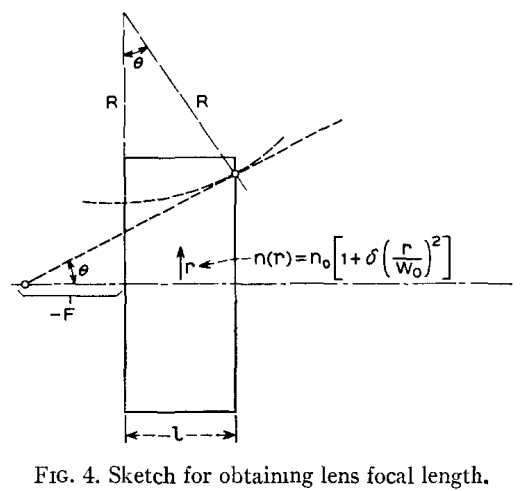
\includegraphics[width=0.6\textwidth]{./files/gordon_lens.png}
    \caption{Lentille équivalente pour une cellule de largeur $l$ d'indice parabolique dans laquelle un rayon lumineux se propage en arc de cercle. Extrait de Gordon \emph{et al} \cite{gordon_longtransient_1965}. $R$ est le rayon de courbure de la trajectoire du rayon lumineux, $\theta$ est l'angle d'un rayon d'incidence nulle après la lentille élémentaire, $F$ est la distance focale (que je note $f'$ distance algébrique focale image par la suite), $w(z)$ est la demie largeur à 1/e du faisceau gaussien. Dans l'approximation des petits angles et pour une cellule fine, on trouve $F = rR/l$ et $\frac{1}{R} = \frac{1}{n}\frac{\mathrm{d}n}{\mathrm{d}r}$.
    \label{FIGgordonlens}}
    \end{figure}


\subsubsection{Cas d'une cellule fine}\label{cellulefine}

Dans cette partie, j'explique le résultat des papiers de Gordon et Whinnery que j'utilise par la suite dans la simulation numérique. Il s'agit de calculer la focale d'une cellule fine d'épaisseur $l$ traversée par un faisceau gaussien. Le différentiel de température par rapport à l'équilibre $\Delta T(r,t)$ est décrit par l'équation de diffusion ($c$ capacité thermique, $\rho$ masse volumique, $k$ diffusivité thermique) :

$$
c\rho\frac{\partial}{\partial t}[\Delta T(r,t)] = \dot{q}(r) + k \nabla^2[\Delta T(r,t)]
$$

Le terme source $q$ de l'équation lié à l'absorption du faisceau de puissance $P$ par le milieu de coefficient d'absorption $\alpha$ vaut \cite{gordon_longtransient_1965} :

$$
\dot{q}(r) = \frac{\alpha P}{\pi w^2_z}\exp \left(\frac{-2r^2}{w^2_z} \right)
$$

Ce qui donne une solution de la forme \cite{gordon_longtransient_1965} :

$$
\Delta T(r,t) = \frac{\alpha P}{4\pi k} \int_0^t \left( \frac{1}{1+2t'/t_c} \right) \exp \left( \frac{-2r^2/w_z^2}{1+2t'/t_c} \right) \mathrm{d}t'
\quad \text{où} \quad
t_c = \frac{w_z^2}{4k}
$$

Dans notre cas, on se contentera de l'approximation au premier ordre de cette solution \cite{gordon_longtransient_1965} :

$$
\Delta T(r,t) \simeq \frac{\alpha P}{4\pi k} \left[ \ln\left( 1+\frac{2t}{t_c} \right) - \frac{2(r^2/w_z^2)}{1+t_c/2t} \right]
$$

Le premier terme est indépendant de $r$ et correspond au réchauffement progressif global de la tranche de liquide. De plus, il est de plus en plus lent à mesure que l'on s'éloigne du waist et se retrouve dominé par les conditions aux limites et par la diffusion le long de l'axe ici non exprimées. On peut donc l'ignorer \cite{gordon_longtransient_1965} pour simplifier le calcul sans altérer le résultat. On a donc :

$$
\Delta T(r,t) = \Delta T_\infty \frac{1}{1+t_c/2t}
\quad \text{où} \quad
\Delta T_\infty = \Delta T(r,t_\infty) = -\frac{\alpha P}{2\pi k}\frac{r^2}{w_z^2}
$$


Si l'on suppose constant le coefficient de variation de l'indice optique ($\mathrm{d}n/\mathrm{d}T$), on a donc un profil d'indice quadratique en $r$ :

$$
n(r,z) = n_0 + \frac{\mathrm{d}n}{\mathrm{d}T}\Delta T = n_0 \left( 1+ \delta_t (r/w_z)^2 \right)
\quad \text{où} \quad
\delta_t = - \frac{\mathrm{d}n}{\mathrm{d}T} \frac{\alpha P}{2\pi kn_0} \frac{2}{1+t_c/2t}
$$

Pour un profil d'indice quadratique tel que celui-ci et dans l'approximation des lentilles minces, on peut définir la distance focale équivalente (Fig. \ref{FIGgordonlens}):

$$
f' = -\frac{w^2_z}{2ln_0\delta_t}
$$

Cela permet d'établir la valeur de la focale $F$ au cours du temps :

$$
f'(t) = f'_\infty \left( 1 + \frac{t_c}{2t} \right) \quad
\text{où} \quad f'_\infty = \frac{\pi k w_z^2}{\alpha Pl(\mathrm{d}n/\mathrm{d}T)}
$$

On a donc une valeur de la focale $f'$ d'une tranche de liquide d'épaisseur $l$. Dans un premier temps, intéressons-nous au régime stationnaire à $t_\infty$.

\begin{figure}
    \centering
    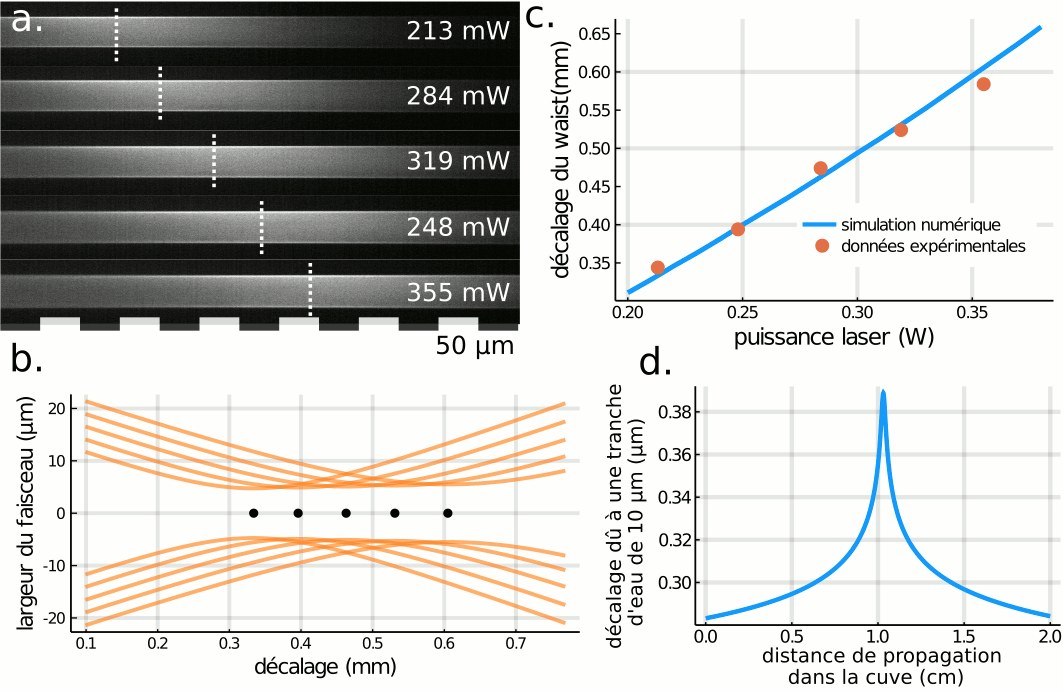
\includegraphics[width=\textwidth]{./files/thermal_shift_model.svg.png}
    \caption{Effet de lentille thermique. La propagation dans l'eau d'un faisceau intense induit un gradient de température et donc un gradient d'indice qui dévie les rayons et décale le waist.
    \\ a. Feuille de lumière imagée dans la fluorescéine pour plusieurs puissances laser différentes. La position mesurée du maximum d'intensité est marquée par un trait pointillé.
    \\ b. Simulation numérique pour les mêmes puissances. La demie largeur du faisceau est calculée pour chaque pas de propagation. La largeur minimale du faisceau selon la simulation est marquée par un point. On remarque par ailleurs que cette largeur minimale augmente avec la puissance.
    \\ c. Comparaison des valeurs expérimentales montrées précédemment avec une simulation numérique réalisée pour des puissances comprises entre 0.2 et 0.38 W.
    \\ d. Contribution de chaque tranche de liquide d'épaisseur 10 µm au décalage du waist pour un faisceau de 0.2 W. La contribution maximale a lieu autour du waist, après 1 cm de propagation plus 0.35 mm de décalage.
    \label{FIGthermalfluorescine}}
    \end{figure}

\subsubsection{Simulation numérique}\label{simuthermallens}

Pour décrire la propagation du faisceau à travers un milieu épais, on le divise en éléments fins.
On part du principe que le faisceau reste gaussien tout au long du parcours, il peut donc être entièrement décrit pour chaque $z$ par la position et la largeur de son waist. Pour chaque tranche de liquide d'épaisseur $l$, on applique l'effet de la lentille équivalente dont la focale est définie suivant la partie précédente pour trouver le déplacement du waist et son élargissement. La figure \ref{FIGthermalfluorescine} montre le résultat de cette simulation comparé à une mesure expérimentale. Le code de la simulation est présenté en annexe \ref{APPsimuthermallens}. Les valeurs numériques utilisées sont fournies en annexe \ref{paramvalue}.

Lorsqu'on augmente la puissance laser, la largeur du waist augmente, ce qui étale l'intensité lumineuse sur une plus grande surface. Au-dessus d'une puissance limite, l'effet résultant est une diminution de l'intensité maximale, et donc de l'effet deux photons. La valeur expérimentale de cette puissance limite est d'environ 0.4 W (on retrouve également cette valeur par simulation \ref{AppFIGmaxintensity}).

Chaque tranche de liquide d'épaisseur $l$ apporte une contribution différente au décalage du point focal. La contribution relative de chaque lentille élémentaire dépend de deux phénomènes ayant un effet opposé l'un de l'autre. Plus l'on s'approche du waist, plus le gradient de température est fort, et plus la lentille est divergente, ce qui augmente la contribution au décalage. Au contraire, plus on s'approche du waist (au sens de Rayleigh), moins le faisceau est convergent, ce qui diminue la contribution au décalage. Finalement, la contribution au niveau du waist est légèrement plus élevée qu'en dehors (\ref{FIGthermalfluorescine} d.).

% OK VolkerComment2
% Make a plot that shows the contribution of every lens element as a function of the distance to the focal point.

\subsection{Effet dynamique}

\subsubsection{Temps caractéristique}

L'effet de lentille thermique a une composante dynamique liée au temps d'établissement de l'équilibre de température. Cet effet a un temps caractéristique $t_c = \frac{w_z^2}{4D}$ qui dépend uniquement de la largeur du faisceau (on considère constante $k = 1.43\times 10^{-7} m^2/s$ la diffusivité thermique de l'eau). Au début de la propagation dans la cuve, le faisceau est large (1 mm), ce qui donne un temps caractéristique de l'ordre de plusieurs secondes. Près du waist, au contraire, ce temps est très court, de l'ordre de la microseconde. Il faut donc réaliser une simulation pour estimer la dynamique du système complet. 
% IGN modèle Tom
En pratique, on constate un temps d'établissement de l'ordre de la seconde.
% IGN mesures établissement

\subsubsection{Solutions}\label{solutionseffetthermique}

Lorsque l'eau bouge dans la cuve, l'équilibre thermique est rompu et il faut attendre quelques temps caractéristiques avant de retrouver l'équilibre. Pendant ce temps, le waist du laser se déplace et change l'illumination de l'échantillon. C'est le phénomène dont les effets ont empêché les premières acquisitions. Une première solution consiste à moins chauffer le milieu pour minimiser l'effet de lentille thermique. Pour cela, j'ai mis en place un obturateur piloté pour éteindre le laser en dehors des périodes d'acquisition. En illuminant pendant 10 ms d'exposition et en coupant pendant 90 ms de pause, on diminue ainsi par dix la puissance moyenne, et donc l'échauffement. Cela impose une contrainte forte sur la fréquence d'acquisition, mais m'a permis de réaliser des enregistrements.
Comme le décalage du waist est en première approximation proportionnel à la longueur traversée, une deuxième solution pour le réduire est de concevoir une cuve dans laquelle l'épaisseur d'eau traversée est plus fine. Je n'ai pas testé cette solution.
Une troisième solution est de diminuer le taux de répétition du laser, comme indiqué en partie \ref{SECTIONconcentrationtemporelle}. Cette solution nécessite un autre laser, je ne l'ai pas explorée.


\section[Tangage deux photons]{Feuille de lumière deux photons lors d'une stimulation en tangage}

En section \ref{SECTIONtiltmicroscope1P}, je présente un microscope adapté à une stimulation vestibulaire en tangage. Avec la fibre présentée précédemment, j'ai pu utiliser ce montage pour une imagerie deux photons. Je présente ici les résultats.

\subsection{Difficultés supplémentaires rencontrées}

Outre les défis techniques cités précédemment concernant la fibre optique et l'effet thermique, les acquisitions deux photons ont révélé certaines difficultés supplémentaires avant de reproduire les résultats obtenus en un photon.

\subsubsection{Phototoxicité}

\paragraph{Photoblanchiment et saturation du rapporteur calcique}
Je n'ai observé aucune limite liée au photoblanchiment du rapporteur calcique ni à la saturation. Ces phénomènes apparaissent en un photon quand l'intensité absorbée par le fluorophore dépasse un certain seuil. Ce seuil n'a pas été atteint dans mon expérience.

\paragraph{Éviter les yeux}
Le laser un photon pénètre les zones transparentes mais est absorbé par les zones opaques comme les yeux. Cela éblouit le poisson et crée une zone d'ombre, mais n'endommage pas la larve, car les puissances en jeu sont relativement faibles (1-10 mW en continu). Le laser deux photons fonctionne à des puissances moyennes bien plus élevées (100-1000 mW) nécessaires à l'effet deux photons. À ces niveaux de puissance, la moindre absorption génère un échauffement intense qui détruit instantanément les tissus biologiques. C'est notamment le cas des yeux qui carbonisent immédiatement si le laser les touche. Pour réaliser des enregistrements du volume entier, il a donc fallu procéder en plusieurs étapes : d'abord la partie supérieure entière, puis la partie inférieure en excluant les yeux. 

\paragraph{Cavitation}
Si une zone transparente du tissu présente un niveau d'absorption légèrement trop élevé, la chaleur s'y accumule et donne lieu à un phénomène de cavitation. Une bulle de gaz se forme alors et grossit en déformant tous les tissus alentour, et en augmentant localement l'absorption. Si l'on augmente l'énergie des impulsions, le phénomène de cavitation apparaît plus facilement et s'auto-entretient. Le degré de phototoxicité augmente avec l'énergie portée par une impulsion. Même à énergie plus faible, il est possible que le laser touche un pigment et déclenche la cavitation.

\subsubsection{Rapport signal à bruit}
Le niveau de signal obtenu dans les enregistrements deux-photons est bien plus faible que dans les enregistrements un-photon. Avec les paramètres finaux (exposition, binning, puissance laser, lignées transgéniques...) la valeur d'un pixel de caméra correspondant à un neurone est de l'ordre de 2000 en un-photon et 800 en deux-photons, pour un niveau de bruit de 400 (le niveau de bruit pour un pixel est de 100, soit 400 après binning par 4 pixels). Un pixel correspondant à l'autofluorescence des tissus est autour de 600 en un-photon et tombe sous le niveau de bruit en deux-photons. Un rapport signal à bruit si faible pose plusieurs problèmes.
\paragraph{Alignement sur le cerveau de référence}
Un cerveau imagé en deux photons apparaît assez différent d'un cerveau en un photon. J'ai donc réalisé un cerveau de référence en deux photons dans l'espace de référence du laboratoire. Malgré cela, pour un rapport signal à bruit trop faible, l'alignement automatique sur le cerveau de référence est impossible. J'ai donc dû faire la plupart des alignements à la main en utilisant le logiciel 3DSlicer.
\paragraph{Moyennage des cartes de phase}
Calculer une carte de phase moyenne nécessite de moyenner séparément la partie réelle et la partie imaginaire du nombre complexe obtenu au pic de la transformée de Fourier. Cependant, pour un niveau de signal faible, le rapport signal à bruit peut largement varier d'une expérience à l'autre. On doit donc appliquer une égalisation de contraste dépendant du module du nombre complexe.
% IGN écrire le programme pour faire une égalisation de contraste permettant de moyenner

\subsubsection{Enregistrements en plusieurs étapes}
Comme on l'a vu en partie \ref{solutionseffetthermique}, la solution adoptée en attente de mieux est de faire des pauses entre deux expositions pour diminuer l'intensité moyenne absorbée. Cela contraint la fréquence d'acquisition des images. Pour conserver une fréquence de 2.5 Hz pour chaque couche, j'ai donc dû réduire le nombre de couches à 4. Chaque volume est donc enregistré non pas en une fois mais en plusieurs. Si à un moment le laser touche un œil, le poisson est détruit et les enregistrements ultérieurs sont compromis. J'ai donc finalement réalisé assez peu d'acquisitions valides.
% 11 ms exposition
% 89 ms pause
% ×4 = 400 ms

\subsection{Comparaison de l'imagerie 1P/2P}

\begin{figure}
    \centering
    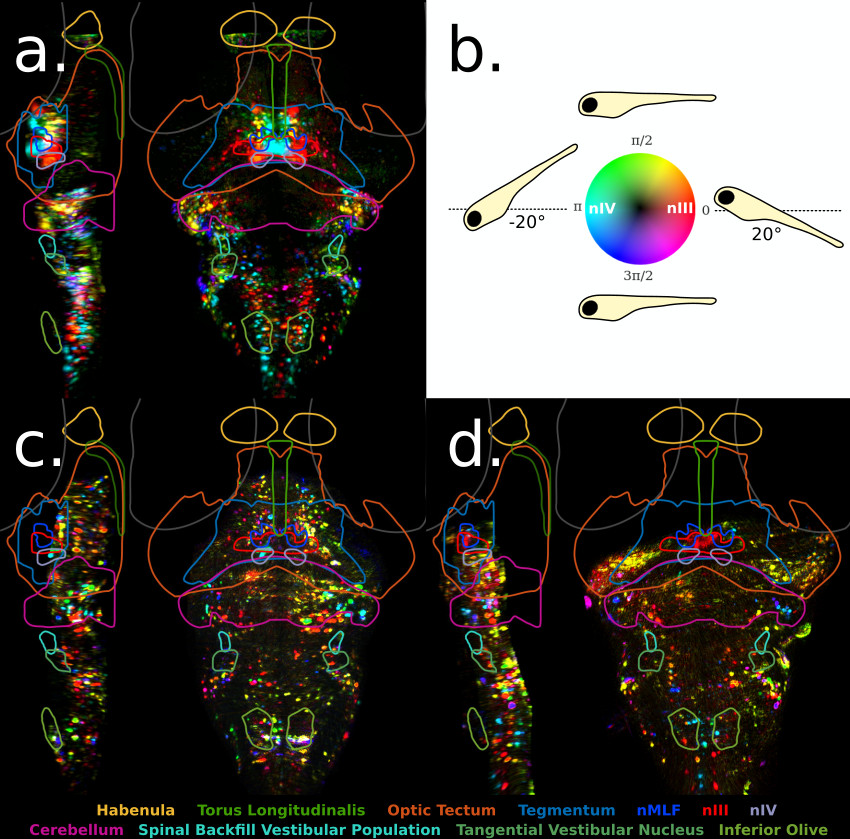
\includegraphics[width=\textwidth]{./files/1P-2P.svg.jpg }
    \caption{Comparaison entre l'acquisition un photon (1P) et deux photons (2P) en imagerie statique et dynamique.
    \\ a. Carte de réponse pour une stimulation en tangage imagée en 1P déjà montrée en figure \ref{FIGtiltroll}.
    \\ b. Légende des couleurs de la carte. Les noyaux nIII et nIV sont notés sur leur couleur dominante à titre indicatif.
    \\ c, d. Cartes de réponse pour une stimulation en tangage imagée en 2P. En (b.) seule la partie supérieure du cerveau est imagée, en (c.), seule la partie inférieure est imagée.
    \label{FIG1P2P}}
    \end{figure}

\subsubsection{Résultats}

La figure \ref{FIG1P2P} montre des cartes de phase obtenues en un photon (a.) et en deux photons (c,d.). En (c.), l'enregistrement a été réalisé en quatre étapes de quatre couches, mais pendant la dernière étape, l'œil du poisson a été touché par le laser, ce qui a rendu les données inexploitables. Seules les trois premières étapes apparaissent donc, et les régions profondes comme les noyaux oculomoteurs ne sont pas visibles. En (d.), le laser était plus loin des yeux, ce qui a permis d'enregistrer également les couches profondes sans les endommager. Les noyaux nIII et nIV sont cependant légèrement tronqués. Les réponses obtenues sont globalement très semblables en 1P et 2P.

Ces cartes de phase sont une preuve de faisabilité pour le microscope deux photons rotatif appliqué à une stimulation vestibulaire.

\subsubsection{Conclusion}

Malgré les difficultés techniques rencontrées, j'ai pu réaliser un microscope rotatif capable de réaliser l'acquisition deux photons de l'activité du cerveau de la larve pendant une stimulation en tangage. Quelques améliorations sont à apporter pour augmenter la fréquence d'acquisition et empêcher le laser d'atteindre l'œil. On peut par exemple diminuer la distance de propagation dans l'eau et diminuer la fréquence de répétition du laser. Cela ouvre la voie à des expériences sur l'intégration visuo-vestibulaire lors du contrôle postural à roulis.